\documentclass[9pt, letterpaper]{article}
\usepackage[margin=.6in]{geometry}
\usepackage[pdftex]{graphicx}

\begin{document}

\begin{center}
{\Large{\bf Visual Analytics Project Proposal}}\\*[3mm]
{\bf A Visual Exploration of Manifold Learning for Images } \\*[3mm]
Prof. Santucci, Dr. Angelini\\
Mattia Stellacci
\end{center}



\section{Proposal}

Manifold learning techniques are not only often used for dimensionality reduction, they are also invaluable tools to visual analytics, allowing data to be expressed in terms  more comprehensible to humans but are also powerful tools for machine learning, counteracting the notorious \textit{curse of dimensionality} and allowing for more simple machine learning systems.  

In their utility to human comprehension and computational robustness they are therefor invaluable tools to any data-/computer Scientist or anyone dealing with large amounts of manifold data. 

I would like to propose a visual analytics system using the well-know MNIST dataset to aid the comprehension, comparison and discrimination of different manifold learning techniques.  Consisting of thousands of 28x28 pixel, bilevel images of handwritten digits, this dataset offers many instances of highly dimensional($28\cdot28= 784$ pixels)  yet (to a human) easliy classifiable data.

The idea is to allow the user to visualize a two-dimensional representation (as calculated by a manifold learning technique of their chosing) on a cartesian plane.A subset of these points in the two-dimensional graph can then be selected by the user and the images they correspond to are displayed. While hovering over individual points reveals the images being represented, selecting a set allows the user to see either the various images in that range, or a combination/aggregation thereof. Aggregations can either be average images calculated by the superpostition of the raw images, or by applying morphology to emphasize similarities or differences.       

\vspace{15pt}

\fbox{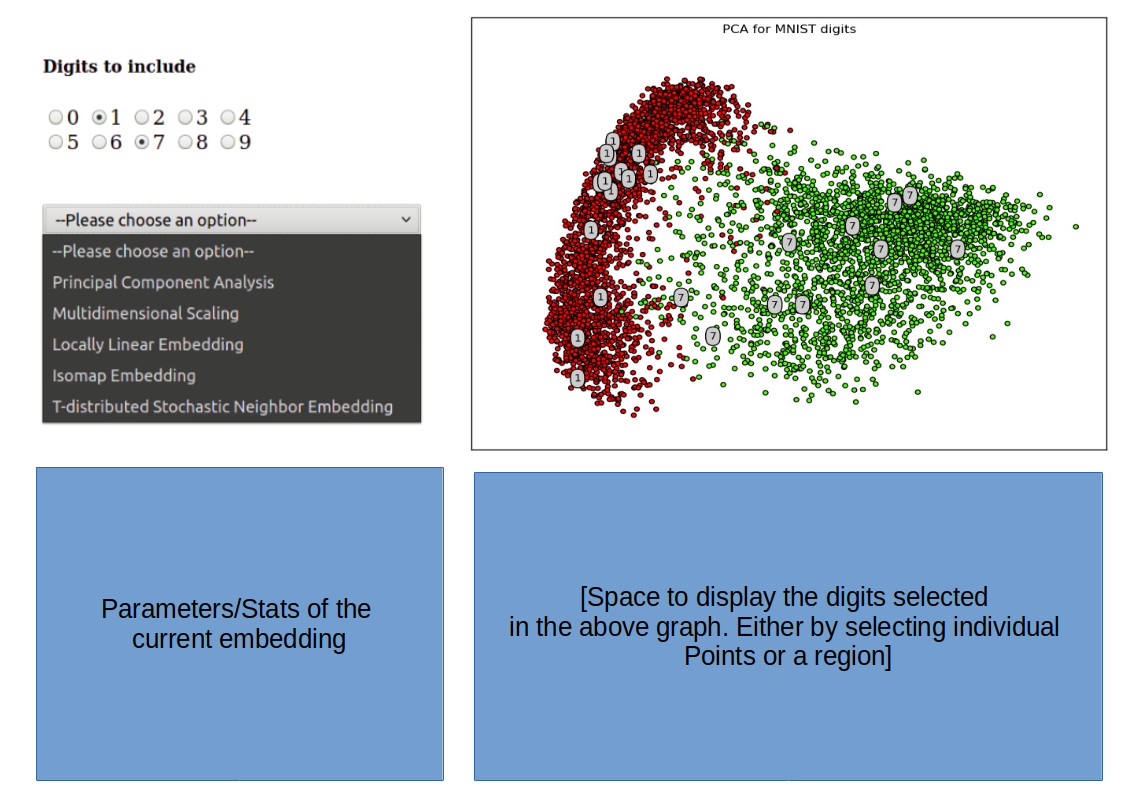
\includegraphics[scale=.5]{mockup_va.png}}

\vspace{15pt}

While similar visualizations are often used as a visual aid while explaining the techniques involved, I have never encountered an interactive implementation where points in the graph can be selected and the raw data they represent visualized. Using \texttt{D3} and a \texttt{WebAssembly} build of \texttt{OpenCV} it is my belief that a powerful visualization can be implemented in the browser to enable people to gain a deeper understanding of dimensionality reduction on images and to understand how the data is distributed across the resulting space. Especially if these methods are to be used as a part of machine learning pipeline, I believe that visualizing their distribution can be an aid to chosing  an adequate classifier and a powerful educational tool. 

\end{document}
